\documentclass[11pt]{article}

\usepackage[a4paper,margin=1in]{geometry}
\usepackage{graphicx}
\usepackage{booktabs}
\usepackage{array}
\usepackage{hyperref}
\usepackage{float}

\title{Understanding CNN vs Vision Transformer:\\
Source-Stage Results on CIFAR-10}
\author{}
\date{March 2026}

\begin{document}

\maketitle

\begin{abstract}
This report summarizes the current source-stage experiments comparing a lightweight convolutional neural network (CNN) and a lightweight Vision Transformer (ViT) trained from scratch on CIFAR-10. The goal is to compare accuracy, data efficiency, robustness to occlusion and texture corruption, and class-level behavior before moving to downstream transfer learning. The main result is clear: in this setup, the CNN is substantially stronger on clean accuracy and low-data learning, while the ViT is markedly more robust to texture corruption. This pattern is consistent with prior literature showing that ViTs tend to require more data or stronger training recipes \cite{dosovitskiy2021image,touvron2021training}, whereas CNNs often rely more heavily on local texture cues \cite{geirhos2019imagenet}.
\end{abstract}

\section{Introduction}
Convolutional neural networks use locality and weight sharing as built-in inductive biases \cite{lecun1998gradient}. Vision Transformers instead tokenize images into patches and model global interactions with self-attention \cite{dosovitskiy2021image}. These differences often lead to different learning behavior: CNNs can work well in small-data settings, while ViTs typically benefit from larger-scale data or stronger pretraining and regularization \cite{dosovitskiy2021image,touvron2021training}. Separately, prior work has shown that standard CNNs can be strongly texture-biased \cite{geirhos2019imagenet}.

This report tests whether these broader trends appear in a controlled from-scratch experiment on CIFAR-10 \cite{krizhevsky2009learning}. The present document covers only the source-stage study. Transfer learning to EuroSAT will be added after this stage.

\section{Methodology}
\subsection{Task and comparison}
Both models were trained for image classification on CIFAR-10. The comparison was designed to answer four questions:
\begin{itemize}
    \item Which model is more accurate on the clean test set?
    \item Which model is more data-efficient?
    \item Which model is more robust to occlusion and texture disruption?
    \item What kinds of class confusions remain after training?
\end{itemize}

\subsection{Models}
The CNN baseline is a compact three-stage architecture with convolution, batch normalization, ReLU, max pooling, global average pooling, dropout, and a linear classifier. The ViT baseline is a lightweight patch-based transformer with patch embedding, learnable positional embeddings, a classification token, and transformer encoder blocks \cite{dosovitskiy2021image}. The goal was not to compare the strongest possible CNN against the strongest possible ViT, but to compare two lightweight models under the same training budget.

\subsection{Interpretability}
The pipeline also generates qualitative explanations for the full-data models. Grad-CAM is used for the CNN \cite{selvaraju2017grad}, and attention rollout is used for the ViT \cite{abnar2020quantifying}. These artifacts are available, but the present report focuses on the quantitative source-stage results.

\section{Experimental Setup}
\subsection{Dataset and preprocessing}
CIFAR-10 contains ten object classes and uses RGB images of size $32 \times 32 \times 3$ \cite{krizhevsky2009learning}. The original training split has 50{,}000 images and the test split has 10{,}000 images. In this project, 5{,}000 images were held out from the original training set for validation, leaving a training pool of 45{,}000 images.

Training preprocessing used:
\begin{itemize}
    \item \texttt{RandomCrop(32, padding=4)}
    \item \texttt{RandomHorizontalFlip()}
    \item \texttt{ToTensor()}
    \item channel-wise normalization with CIFAR-10 statistics
\end{itemize}

Validation and test preprocessing used only tensor conversion and normalization. This keeps evaluation deterministic.

\subsection{Data-efficiency protocol}
Separate runs were trained from scratch using 10\%, 25\%, 50\%, and 100\% of the 45{,}000-image training pool. This corresponds to 4{,}500, 11{,}250, 22{,}500, and 45{,}000 training images respectively. These were independent runs, not progressive continuation runs.

\subsection{Robustness protocol}
Robustness was evaluated using the 100\% models only. Two test-time distribution shifts were applied:
\begin{itemize}
    \item \textbf{Occlusion}: a square patch is masked.
    \item \textbf{Texture modification}: local patches are shuffled and perturbed with noise while preserving the global image layout.
\end{itemize}

\subsection{Training details}
All reported CIFAR experiments were trained for 100 epochs with AdamW, learning rate $10^{-3}$, weight decay $10^{-4}$, batch size 128, and seed 42. All values in this report come from one controlled split and one random seed.

\section{Results}
\subsection{Clean accuracy and efficiency}
Table~\ref{tab:main-results} shows the main full-data comparison. The CNN reached 85.7\% test accuracy, while the ViT reached 73.36\%. The CNN therefore outperformed the ViT by 12.34 percentage points while using far fewer trainable parameters (0.37M vs 1.80M). It also trained slightly faster.

This result indicates that, in the current from-scratch CIFAR-10 setting, the CNN is the stronger source-stage model. The weaker ViT performance is consistent with prior work showing that transformers in vision tend to need larger-scale pretraining or more specialized data-efficient training recipes \cite{dosovitskiy2021image,touvron2021training}.

\begin{table}[H]
\centering
\caption{Full-data comparison on CIFAR-10. Macro-F1 values come from checkpoint-based evaluation.}
\label{tab:main-results}
\begin{tabular}{lcccccc}
\toprule
Model & Params & Clean Acc. & Macro-F1 & Occluded Acc. & Texture Acc. & Train Time \\
\midrule
CNN & 374{,}282 & 85.70\% & 0.858 & 80.32\% & 32.98\% & 13m 56s \\
ViT & 1{,}803{,}850 & 73.36\% & 0.733 & 68.81\% & 50.26\% & 15m 46s \\
\bottomrule
\end{tabular}
\end{table}

\subsection{Data efficiency}
The data-efficiency trend is consistent across all fractions. The CNN outperformed the ViT at every training budget:

\begin{table}[H]
\centering
\caption{Test accuracy across training fractions.}
\label{tab:data-efficiency}
\begin{tabular}{lcccc}
\toprule
Model & 10\% & 25\% & 50\% & 100\% \\
\midrule
CNN & 65.70\% & 75.08\% & 81.48\% & 85.70\% \\
ViT & 53.53\% & 60.27\% & 67.03\% & 73.36\% \\
\bottomrule
\end{tabular}
\end{table}

The CNN had a strong early gain from 10\% to 25\% data (+9.38 points), then continued to improve as more data was added. The ViT also improved steadily, but remained behind at every fraction. The gap between the two models stayed large: 12.17 points at 10\% data, 14.81 points at 25\%, 14.45 points at 50\%, and 12.34 points at 100\%.

This confirms that the CNN is more data-efficient in this setting. The ViT did not close the gap even after 100 epochs, which supports the interpretation that the current ViT setup still wants more data or stronger optimization support.

\begin{figure}[H]
\centering
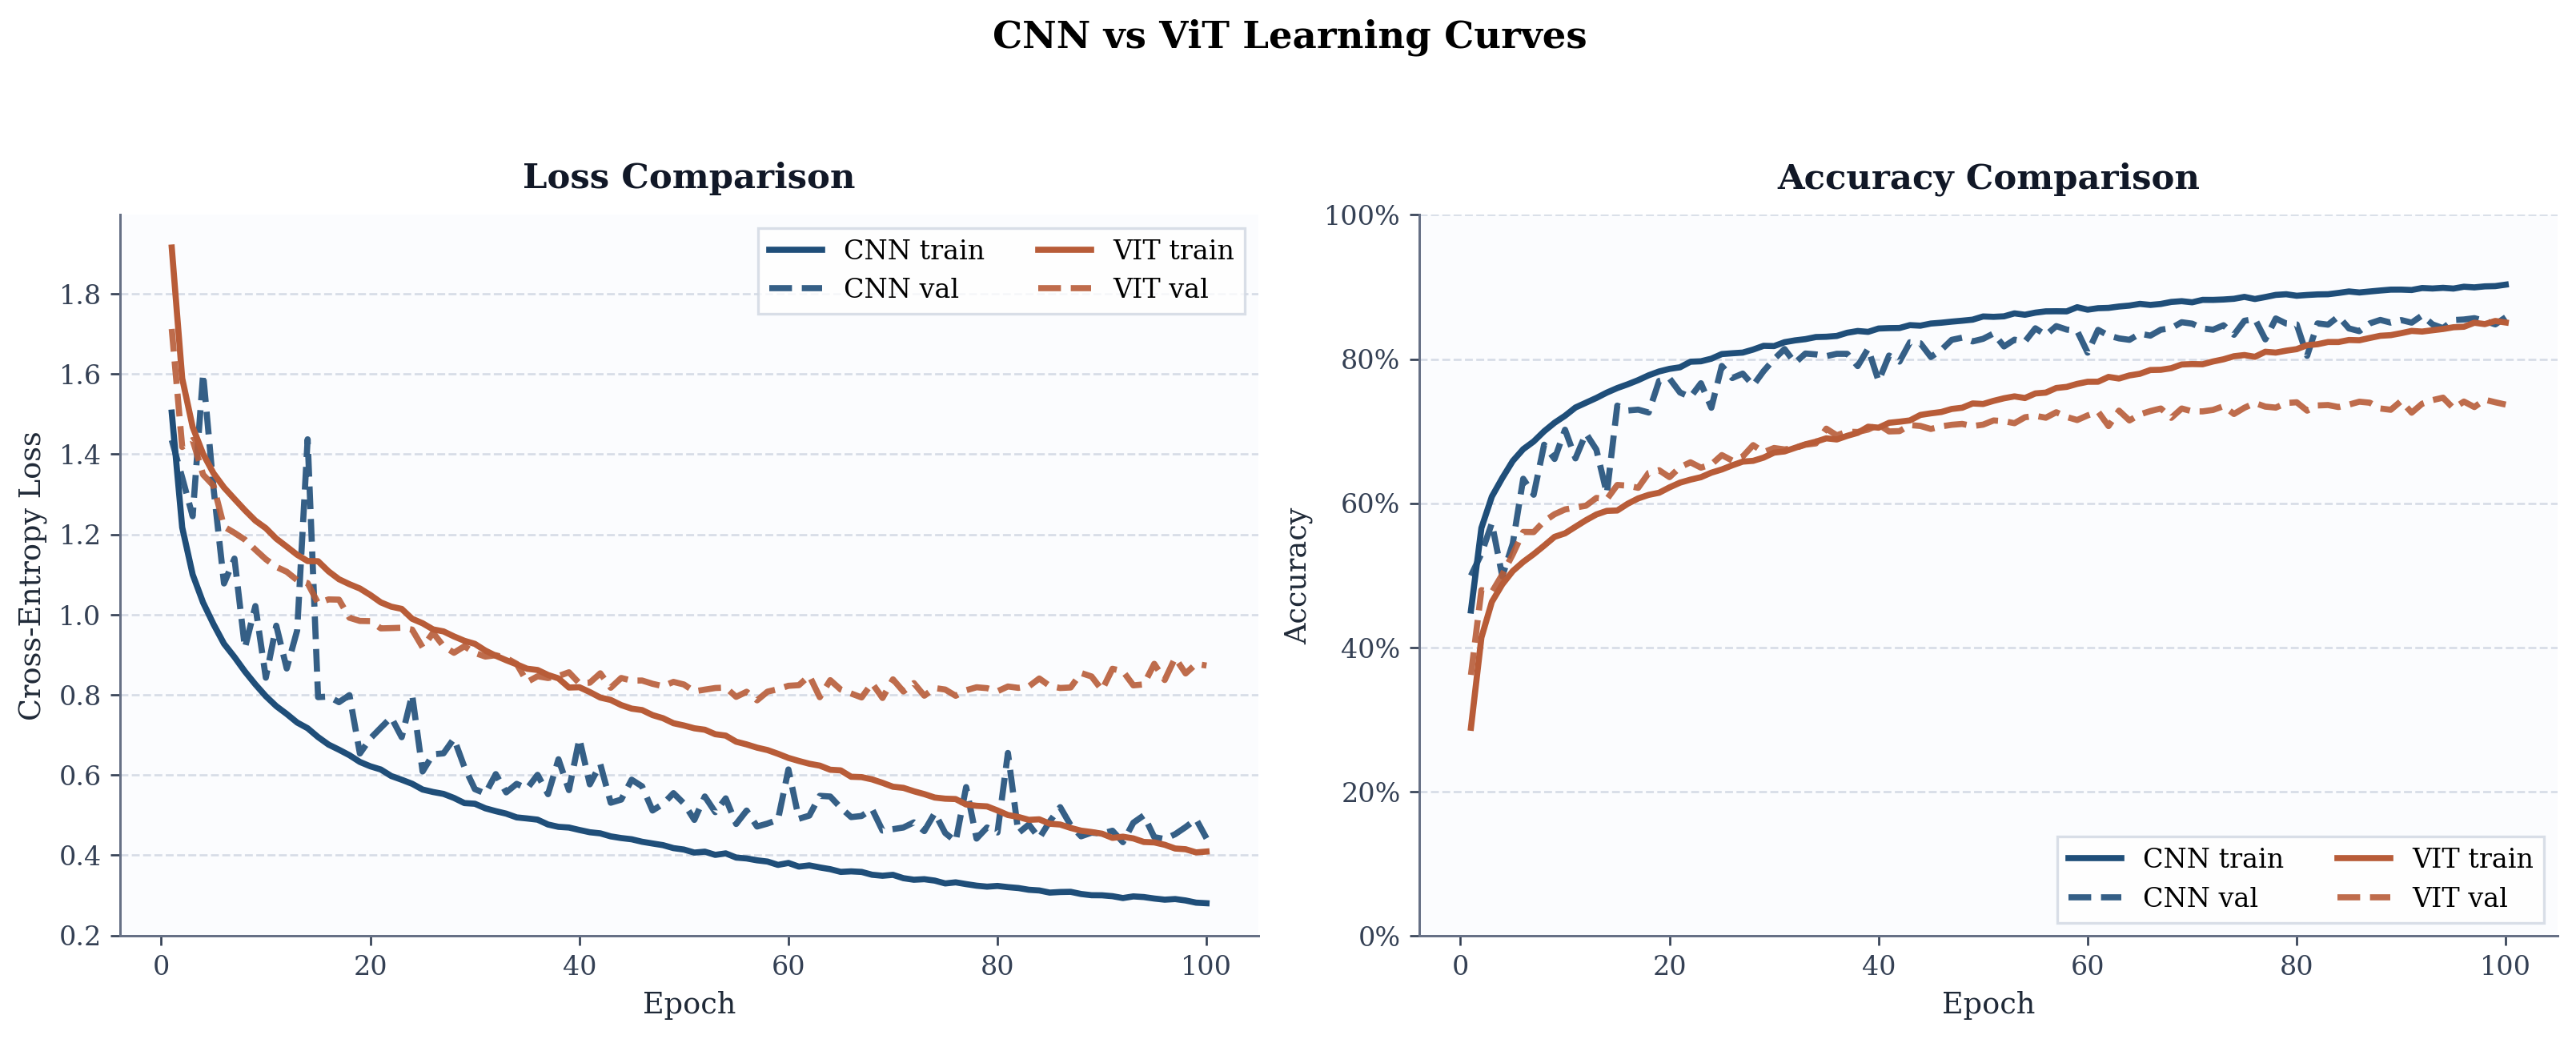
\includegraphics[width=0.82\linewidth]{outputs/plots/cnn_vit_training_comparison.png}
\caption{Shared learning curves for the full-data CNN and ViT runs. The CNN converges faster and to a higher validation accuracy.}
\label{fig:combined-curves}
\end{figure}

\begin{figure}[H]
\centering
\begin{minipage}{0.48\linewidth}
    \centering
    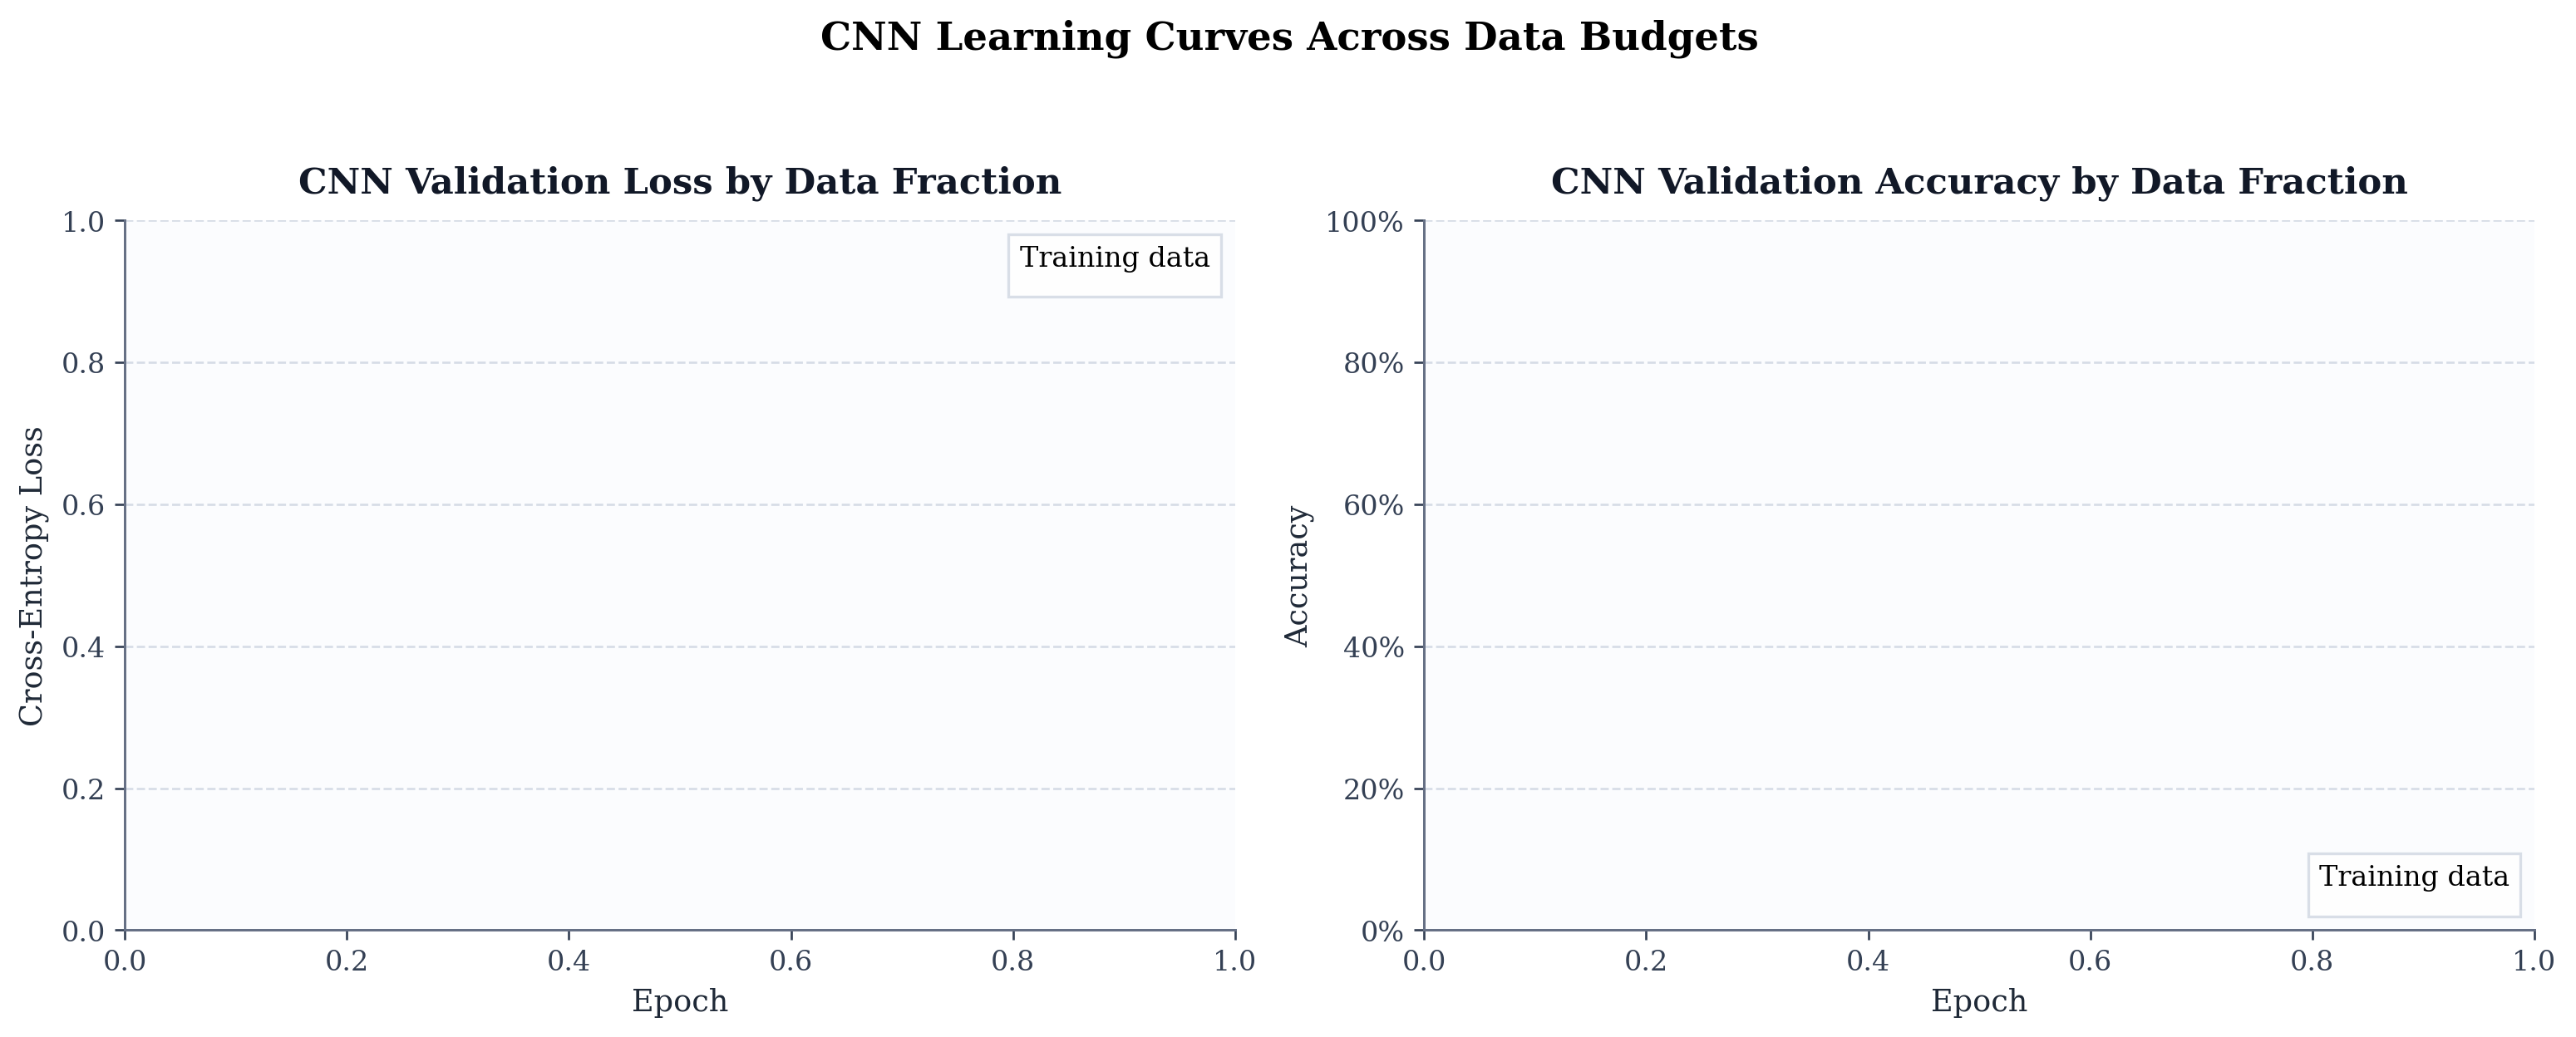
\includegraphics[width=\linewidth]{outputs/plots/cnn_data_fraction_curves.png}
    
    {\small (a) CNN across data fractions}
\end{minipage}
\hfill
\begin{minipage}{0.48\linewidth}
    \centering
    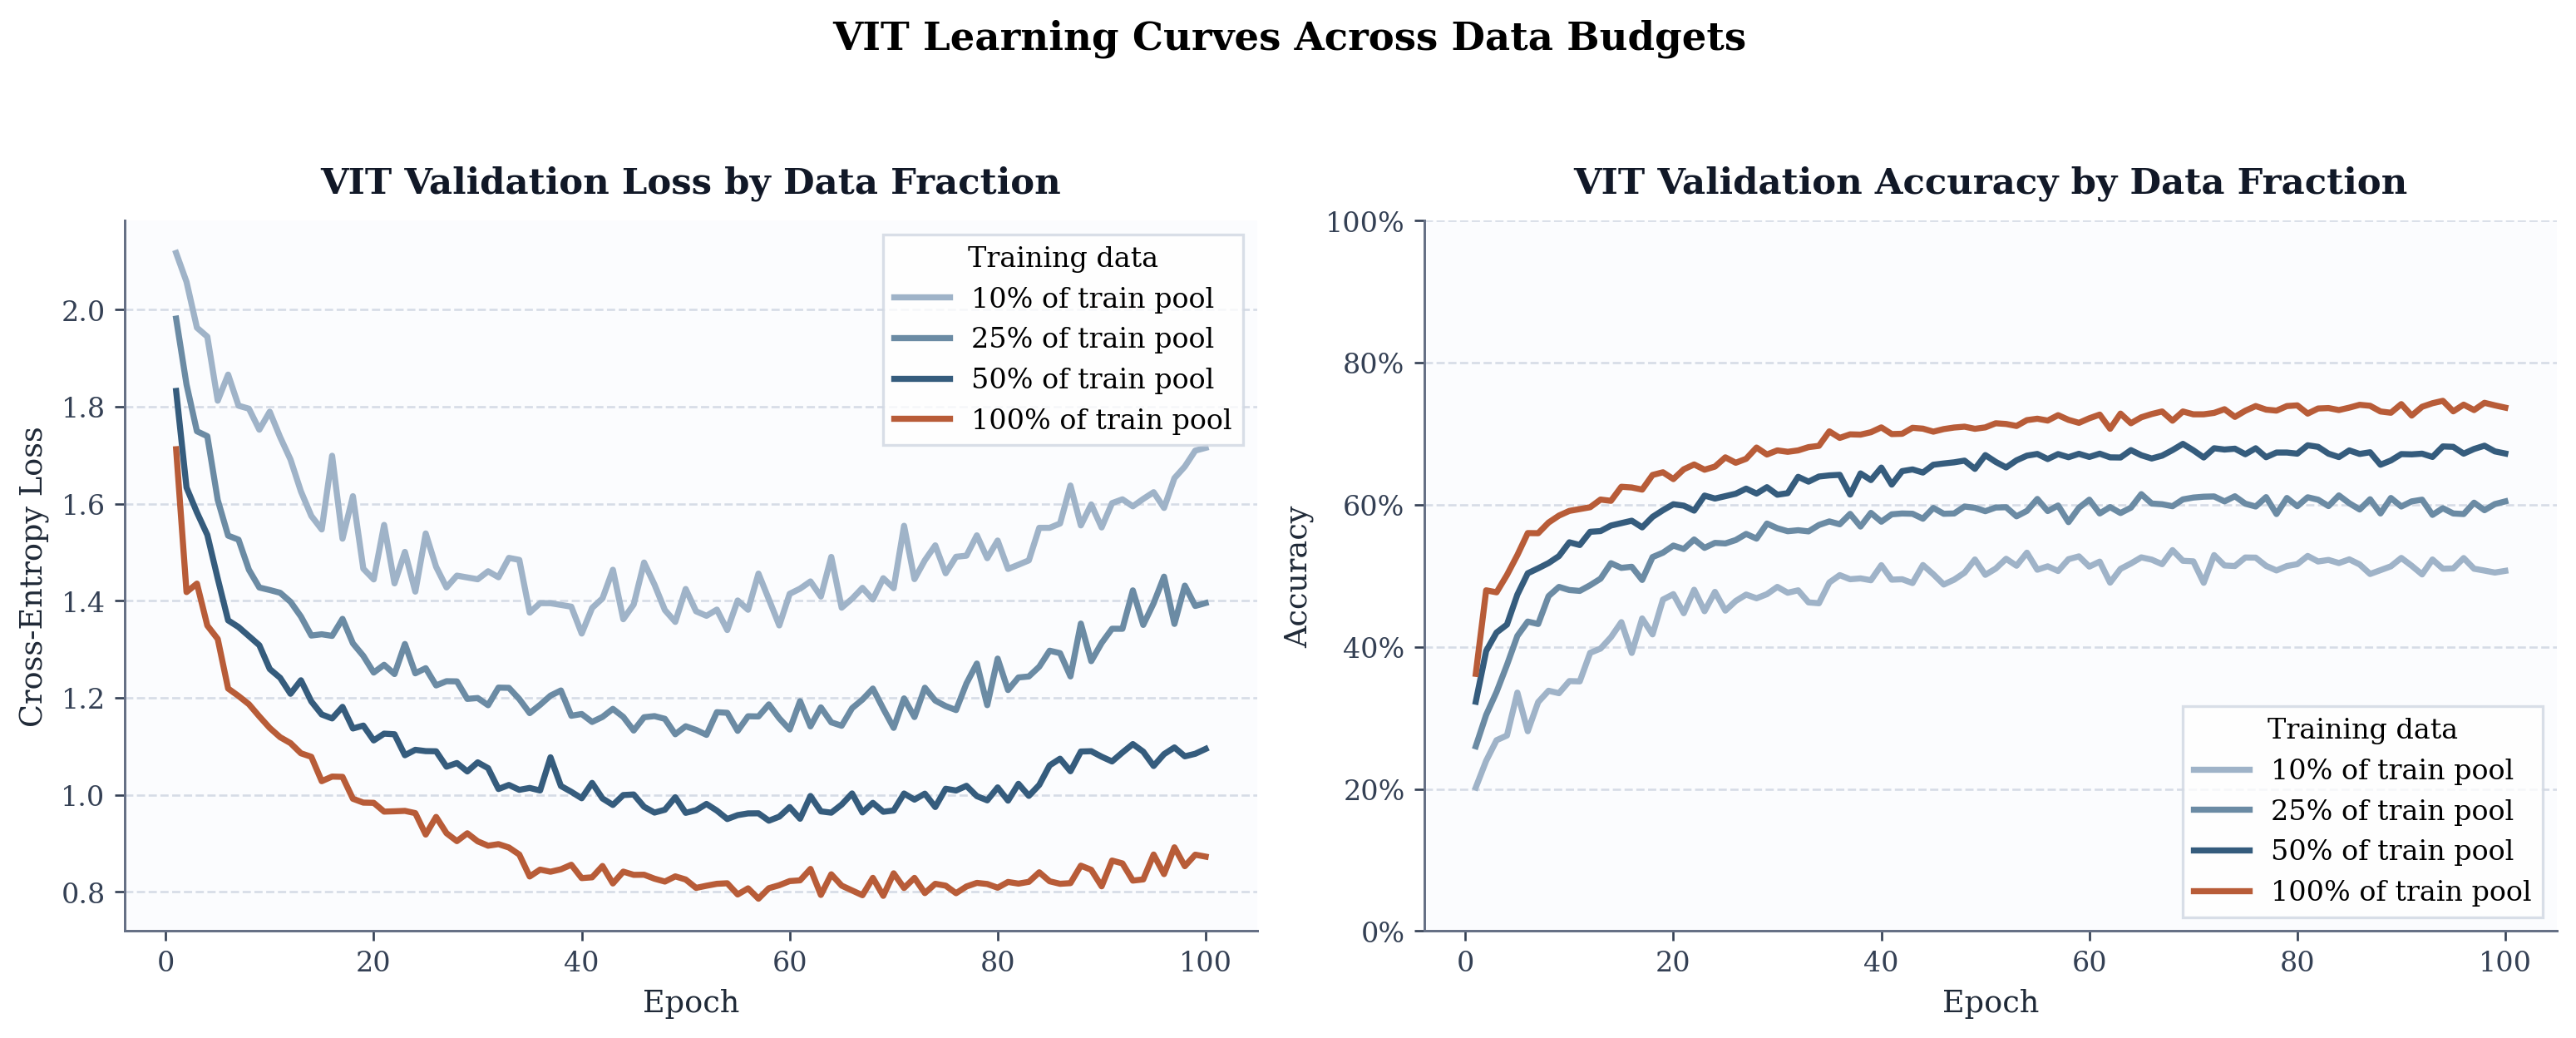
\includegraphics[width=\linewidth]{outputs/plots/vit_data_fraction_curves.png}
    
    {\small (b) ViT across data fractions}
\end{minipage}
\caption{Validation learning curves across data budgets. The CNN remains ahead throughout training, especially in the low-data regime.}
\label{fig:fraction-curves}
\end{figure}

\subsection{Robustness to occlusion and texture modification}
The robustness results are more nuanced than the clean-accuracy results.

Under occlusion, both models degraded moderately:
\begin{itemize}
    \item CNN: 85.70\% $\rightarrow$ 80.32\% (drop of 5.38 points)
    \item ViT: 73.36\% $\rightarrow$ 68.81\% (drop of 4.55 points)
\end{itemize}

The ViT had a slightly smaller drop, but the CNN still retained much higher absolute accuracy.

Under texture modification, the difference was much larger:
\begin{itemize}
    \item CNN: 85.70\% $\rightarrow$ 32.98\% (drop of 52.72 points)
    \item ViT: 73.36\% $\rightarrow$ 50.26\% (drop of 23.10 points)
\end{itemize}

This is the strongest result in the current study. The CNN collapses under texture disruption, while the ViT degrades much less. This pattern is consistent with the texture-bias literature on CNNs \cite{geirhos2019imagenet}. In other words, the CNN is better on standard accuracy, but the ViT appears to rely less heavily on local texture statistics.

\begin{figure}[H]
\centering
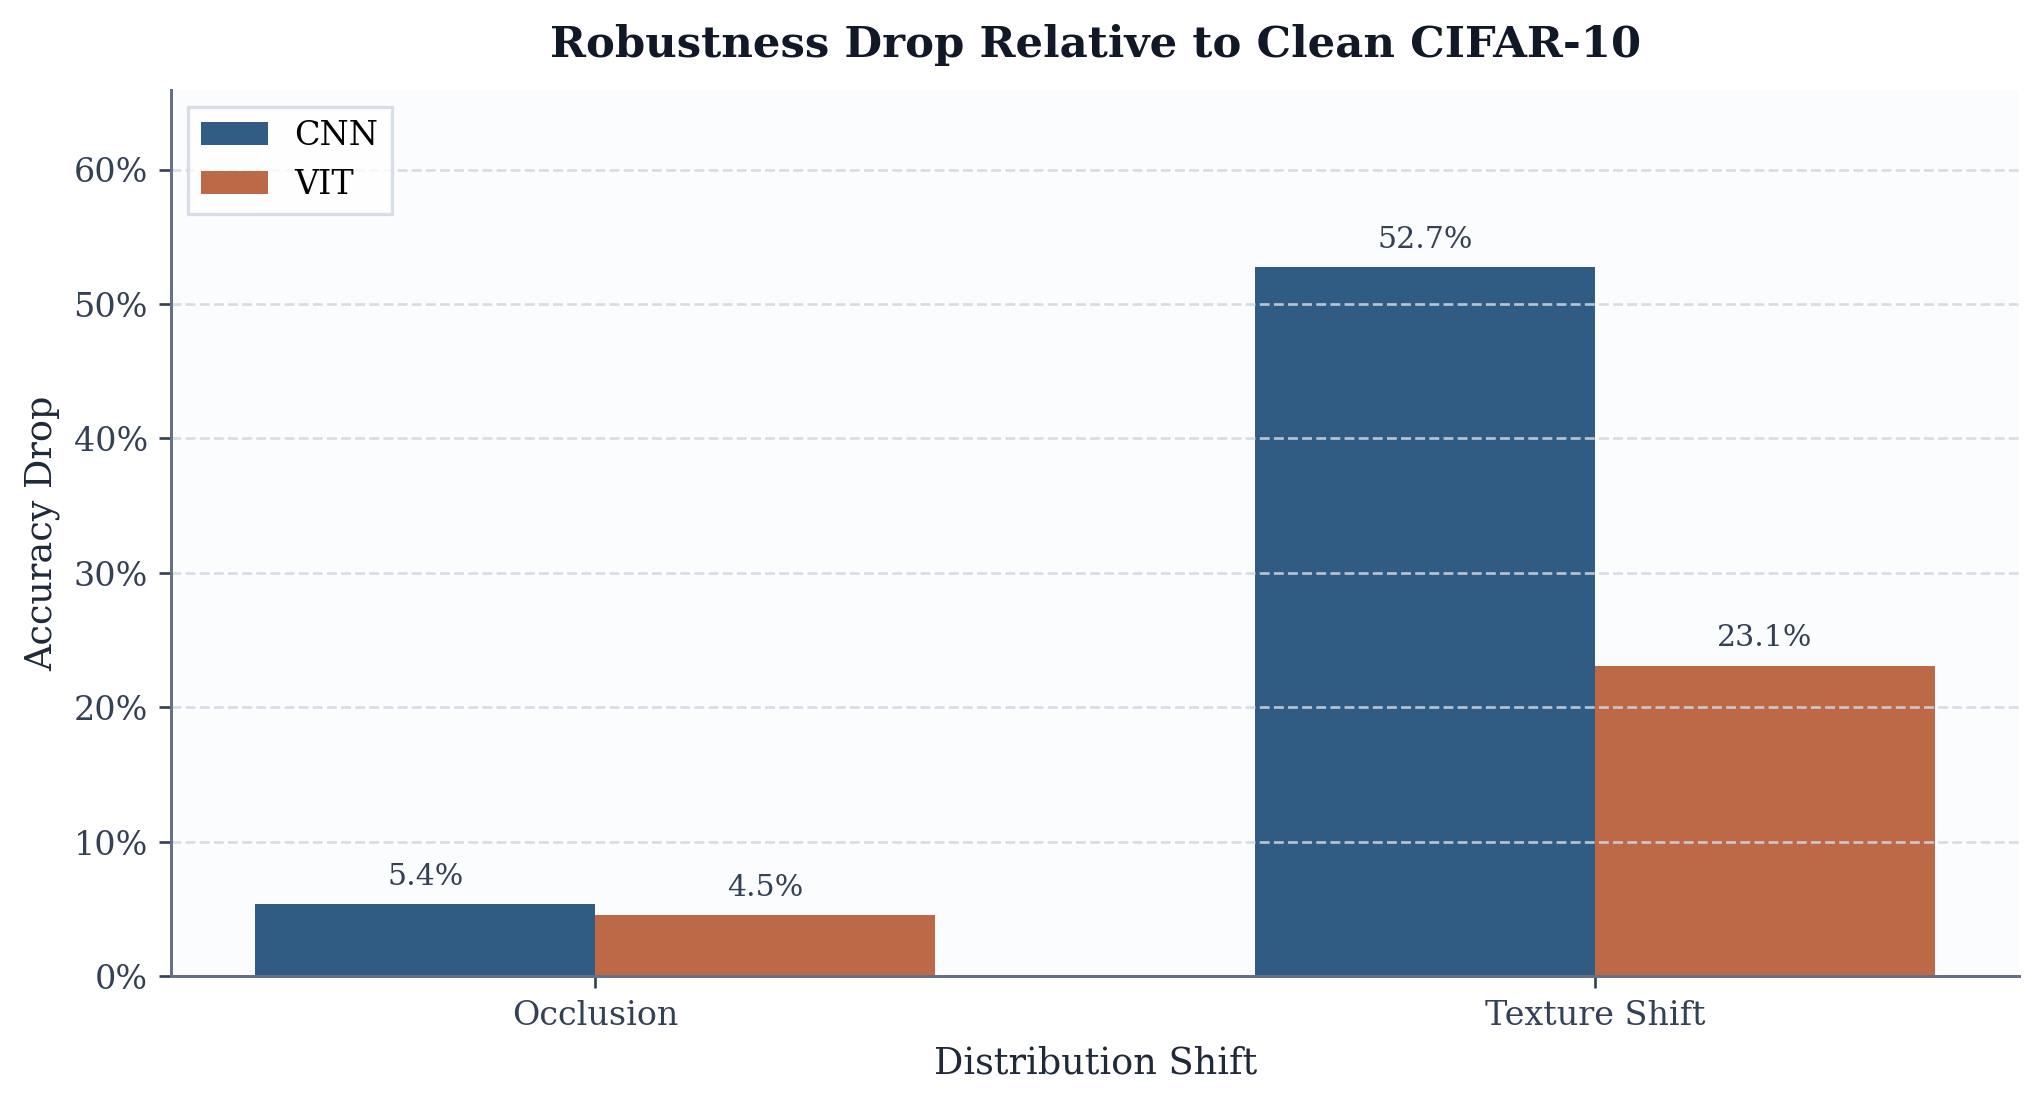
\includegraphics[width=0.72\linewidth]{outputs/plots/robustness_drop.png}
\caption{Accuracy drop relative to the clean CIFAR-10 test set. Texture corruption harms the CNN much more than the ViT.}
\label{fig:robustness}
\end{figure}

\subsection{Class-level behavior}
Checkpoint-based evaluation shows that both models make their largest errors on visually similar animal classes. For the full-data runs:
\begin{itemize}
    \item The CNN's lowest recalls were on \textit{dog} (0.756), \textit{bird} (0.777), and \textit{cat} (0.806).
    \item The ViT's lowest recalls were on \textit{cat} (0.569), \textit{dog} (0.631), and \textit{bird} (0.673).
    \item Both models performed best on vehicle classes, especially \textit{automobile} and \textit{ship}.
\end{itemize}

The dominant confusion pairs also support this interpretation. For the full-data CNN, the largest confusion was \textit{dog} $\rightarrow$ \textit{cat} (156 cases). For the full-data ViT, the largest confusion was also \textit{dog} $\rightarrow$ \textit{cat} (196 cases), with a similarly strong reverse confusion \textit{cat} $\rightarrow$ \textit{dog} (168 cases). These class-level errors suggest that the ViT's main weakness in this experiment is fine-grained discrimination among similar animal categories.

\section{Conclusion}
At the current source stage, the CNN is the better overall classifier on CIFAR-10. It is more accurate, more data-efficient, smaller, and slightly faster. However, the ViT shows a clear advantage under texture corruption, which is important because it suggests a different representation strategy rather than simply a weaker model.

The direct conclusion is therefore not ``CNNs are better than ViTs.'' The more precise conclusion is:
\begin{itemize}
    \item CNN is better for this from-scratch small-image classification setup.
    \item ViT appears less texture-dependent and therefore more robust to the specific texture-shift test used here.
\end{itemize}

This gives a strong foundation for the next stage of the project. The saved 100\% CIFAR checkpoints can now be used for transfer learning on EuroSAT, where the key question will be whether the different source-stage behaviors translate into different downstream transfer performance.

\begin{thebibliography}{9}

\bibitem{lecun1998gradient}
Yann LeCun, Léon Bottou, Yoshua Bengio, and Patrick Haffner.
\newblock Gradient-based learning applied to document recognition.
\newblock \emph{Proceedings of the IEEE}, 86(11):2278--2324, 1998.

\bibitem{krizhevsky2009learning}
Alex Krizhevsky and Geoffrey Hinton.
\newblock Learning multiple layers of features from tiny images.
\newblock Technical report, University of Toronto, 2009.

\bibitem{dosovitskiy2021image}
Alexey Dosovitskiy, Lucas Beyer, Alexander Kolesnikov, Dirk Weissenborn, Xiaohua Zhai, Thomas Unterthiner, Mostafa Dehghani, Matthias Minderer, Georg Heigold, Sylvain Gelly, Jakob Uszkoreit, and Neil Houlsby.
\newblock An image is worth 16x16 words: Transformers for image recognition at scale.
\newblock In \emph{International Conference on Learning Representations}, 2021.

\bibitem{touvron2021training}
Hugo Touvron, Matthieu Cord, Matthijs Douze, Francisco Massa, Alexandre Sablayrolles, and Hervé Jégou.
\newblock Training data-efficient image transformers \& distillation through attention.
\newblock In \emph{International Conference on Machine Learning}, pages 10347--10357, 2021.

\bibitem{geirhos2019imagenet}
Robert Geirhos, Patricia Rubisch, Claudio Michaelis, Matthias Bethge, Felix A. Wichmann, and Wieland Brendel.
\newblock ImageNet-trained CNNs are biased towards texture; increasing shape bias improves accuracy and robustness.
\newblock In \emph{International Conference on Learning Representations}, 2019.

\bibitem{selvaraju2017grad}
Ramprasaath R. Selvaraju, Michael Cogswell, Abhishek Das, Ramakrishna Vedantam, Devi Parikh, and Dhruv Batra.
\newblock Grad-CAM: Visual explanations from deep networks via gradient-based localization.
\newblock In \emph{International Conference on Computer Vision}, pages 618--626, 2017.

\bibitem{abnar2020quantifying}
Samira Abnar and Willem Zuidema.
\newblock Quantifying attention flow in transformers.
\newblock In \emph{Annual Meeting of the Association for Computational Linguistics}, pages 4190--4197, 2020.

\end{thebibliography}

\end{document}
